\chapter{Grundlagen}
\label{sec:grundlagen}


\section{Softwarequalität}
\label{sec:softwarequalität}

Nach der Norm ISO-25000:2014 4.33 bezeichnet der Begriff der Softwarequalität die Fähigkeit einer Software, die expliziten und impliziten Bedürftnisse von Benutzern, unter den Bedingungen unter der sie benutzt wird, zu befriedigen.  \cite {international_organization_for_standardization_iso_so/iec_2014}
Softwarequalität hat nach dieser Definition einen subjektiven Charakter.
Dieser subjektive Charakter macht den Begriff in der Praxis schwer zu greifen und damit nicht direkt anwendbar. Aus diesem Grund existieren sogenannte Qualitätsmodelle, die Softwarequalität messbar und damit auch überprüfbar machen sollen.
Ein solches Qualitätsmodell wird zum Beispiel in der ISO-Norm 9126 vorgestellt. \cite{iso/iec_iso/iec_2001}
Es werden verschiedene Qualitätsmerkmale definiert, die zur Beurteilung der Gesamtqualität eines Softwareprodukts dienen.
Hierunter fallen die Merkmale:

\begin{itemize}
	  \itemsep0pt
      \item Funktionalität
      \item Zuverlässigkeit
      \item Benutzbarkeit
      \item Effizienz
      \item Änderbarkeit
      \item Übertragbarkeit          
\end{itemize}

Es existieren verschiedene Methoden um sicherzustellen, dass Software, bezogen auf die Qualitätsmerkmale gewissen Anforderungen genügt.
Ein Teil der Methoden geht dabei davon aus, dass ein qualitativ hochwertiger Prozess der Produkterstellung die Entstehung von qualitativ hochwertigen Produkten begünstigt.
Das Augenmerk wird hierbei also auf die Prozessqualität gelegt.
Allgemein fasst man diese Gruppe unter dem Begriff prozessorientiertes Qualitätsmanagement zusammen. Die klassischen Vorgehensmodelle der Softwarentwicklung werden z.B. hier eingeordnet.
Worauf sich diese Arbeit jedoch konzentrieren möchte, sind die Methoden des produktorientierten Qualitätsmanagement \cite{prof._dr._r._lindermeier_projekt-_2006}.
Hierbei wird das Softwareprodukt direkt bezüglich der Qualitätsmerkmale überprüft.
Darunter fallen beispielsweise Softwaretests.


\section{Softwaretest}
\label{sec:softwaretest}

Das produktorientierte Qualitätsmanagement unterteilt sich weiter in die Bereiche des konstruktiven und analytischen Qualitätsmanagement.
Unter dem konstruktiven Qualitätsmanagement versteht man den Einsatz von z.B. Methoden, Werkzeugen oder Standards die dafür sorgen, dass ein (Zwischen-)Produkt bestimmte Forderungen erfüllt.
Was man im Allgemeinen aber unter einem Softwaretest versteht, ist im Bereich der prüfenden Verfahren des analytischen Qualitätsmanagement angesiedelt.
Unter analytischen Qualitätsmanagement versteht man den Einsatz von analysierenden bzw. prüfenden Verfahren, die Aussagen über die Qualität eines (Zwischen-)Produkts machen. \cite{prof._dr._r._lindermeier_projekt-_2006} \newline
Die Norm ISO/IEC/IEEE 24765:2010 3.280 definiert das testen von Software als eine dynamische Verifikation des Verhaltens eines Programms, gegen ein erwartetes Verhalten, bei einer endlichen Auswahl an Testfällen. (Im Original: \glqq the dynamic verification of the behavior of a program on a finite set of test cases, suitably selected from the usually infinite executions domain, against the expected behavior.\grqq\ \cite{iso/iec/ieee_systems_2010})
Aufgabe eines Softwaretests ist es dabei nicht, einen Fehler im Code zu Lokalisieren und zu beheben.
Das lokalisieren und Beheben des Defekts ist Aufgabe des Softwareentwicklers und wird auch als Debugging (Fehlerbereinigung, Fehlerkorrektur) bezeichnet.
Während Debugging das Ziel hat, Defekte bzw. Fehlerzustände zu beheben, ist es Aufgabe des Tests, Fehlerwirkungen (die auf Defekte hinweisen) gezielt und systematisch aufzudecken. \cite{spillner_basiswissen_2007}
Dabei dienen definierte Anforderungen als Prüfreferenz, mittels derer ggf. vorhandene Fehler aufgedeckt werden.
\glqq Das Testen von Software dient durch die Identifizierung von Defekten und deren anschließenden Beseitigung durch das Debugging zur Steigerung der Softwarequalität.\grqq\ \cite{spillner_basiswissen_2007}
Als möglicher Rahmen für die Anforderungen können z.B. die in \ref{sec:softwarequalität} bereits beschriebenen Qualitätsmerkmale dienen.


\section{Testprozess}
\label{sec:testprozess}

Der Begriff des Softwaretests, wie er in \ref{sec:softwaretest} beschrieben ist, erfordert eine Einordnung in einen größeren Zusammenhang. Ein Softwaretest steht in der Regel nicht für sich alleine, sondern ist Teil eines größeren Prozesses, der den Softwaretest in seinem gesamten Lebenszyklus begleitet.
Durch den Testprozess wird die Aufgabe des Testens in kleinere Testaufgaben gegliedert.
Splinner und Linz fassen diese Testaufgaben im fundamentalen Testprozess zusammen \cite{spillner_basiswissen_2007}


Testaufgaben, die man dabei unterscheidet sind:

\begin{itemize}
	  \itemsep0pt
      \item Testplanung und Steuerung
      \item Testanalyse und Testdesign
      \item Testrealisierung und Testdurchführung
      \item Testauswertung und Bericht
      \item Abschluss der Testaktivitäten       
\end{itemize}

Obgleich die Aufgaben in sequenzieller Reihenfolge im Testprozess angegeben sind, können sie sich überschneiden und teilweise auch gleichzeitig durchgeführt werden. Diese Teilaufgaben werden im folgenden kurz näher beschrieben. Als Grundlage dient hierfür die Beschreibung des fundamentalen Testprozesses nach Splinner und Linz. \cite[S.20ff]{spillner_basiswissen_2007}

\subsection{Testplanung und Steuerung}
\label{subsec:testplanung_und_steuerung}
Das Testen von Software stellt eine umfangreiche Aufgabe dar. Um diese zu beweltigen wird eine sorgfältig Planung benötigt.
Mit der Planung des Testprozesses wird am Anfang des Softwareentwicklungsprojekts begonnen.
Ziel ist es dabei, die Rahmenbedingungen für die Testaktivitäten festzulegen.
Nachdem Aufgaben und die Zielsetzung der Tests bestimmt wurden, können die Resourcen die für die Durchführung der Aufgaben benötigt werden geplant werden.
Eine weitere Kernaufgabe der Planung ist das Festlegen einer Teststrategie. Da ein vollständiger Test einer Anwendung in der Regel nicht möglich ist, müssen die zu testenden Einheiten nach schwere der Fehlerwirkung priorisiert werden. Je nach schwere der zu erwarteten Auswirkungen, kann dann die Intensität bestimmt werden, mit der ein einzelner Systemteil getestet werden soll.
Ziel der Teststrategie ist es also, eine optimale Verteilung der Tests auf die gesamte Software zu erreichen.
Dabei sind auch geeignete Testendekriterien festzulegen, um zu entscheiden, ob ein Testprozess abgeschlossen werden kann.
Ein weiterer Punkt, der in der Planungsphase berücksichtigt werden muss, ist die Beschaffung von geeigneten Werkzeugen die zur Durchführung und Erstellung der Testfälle benötigt werden.
Die in der Planung erarbeiteten Ergebnisse werden in einem Testkonzept festgehalten.
Eine mögliche Gliederung bietet z.B. die internationale Norm IEEE 829-2008. \cite{ieee_ieee_2008}
Parallel zu den Testaktivitäten muss über den gesamten Testprozess eine Steuerung erfolgen.
Der Fortschritt der Tests und des Projekts wird dabei laufend erhoben, geprüft und bewertet.

\subsection{Testanalyse und Testdesign}
\label{subsec:testanalyse_und_design}
In dieser Phase wird die Testbasis überprüft, also die zugrunde liegenden Dokumente, die für die Erstellung der Testfälle benötigt werden. Spezifikationen und Anforderungen müssen vollständig, konsistent und überprüfbar vorliegen.
Anhand der in der Planung festgelegten Teststrategie und der Testbasis können nun Testfälle erstellt werden.
Die Spezifikation der Testfälle erfolgt dabei in zwei Stufen. Testfälle werden in dieser Phase zunächst recht allgemein definiert. Diese allgemeinen Testfälle können dann später mit tatsächlichen Eingabewerten konkretisiert werden.
Zu der Spezifikation eines Testfalls gehören auch etwaige Rand- und Vorbedingungen sowie ein erwartetes Ergebnis. Um letzteres bestimmen zu können, muss ein so genanntes Testorakel befragt werden. Hierbei handelt es sich um eine Quelle, die auf das erwartete Ergebnis schließen lässt. Ein mögliches Testorakel wäre beispielsweise die Spezifikation der Software.

\subsection{Testrealisierung und Testdurchführung}
\label{subsec:testrealisierung_und_durchführung}
In diesem Schritt des Testprozesses werden aus den allgemein gehaltenen Testfällen konkrete Testfälle gebildet. Diese Testfälle können dann zusammen mit der Testinfrastruktur im Detail realisiert werden. Logisch zusammengehörige Testfälle werden dabei in Testszenarien gruppiert. Dabei ist die in der Planung festgelegte Priorität der Testfälle zu berücksichtigen.
Wenn das Testobjekt zur Verfügung steht, beginnt die Abarbeitung der Testfälle. Jede Durchführung und deren Ergebnisse werden protokolliert. Auf mögliche Abweichungen von den erwarteten Ergebnissen muss entsprechend reagiert werden. Nach der Korrektur des Fehlers ist zu überprüfen, ob der Fehler wirklich beseitigt wurde und bei der Beseitigung keine weiteren Fehlerzustände hinzugekommen sind.

\subsection{Testauswertung und Bericht}
\label{subsec:testauswertung_und_bericht}
In dieser Phase des Testprozesses wird überprüft, ob die in der Planung festgelegten Testendkriterien erfüllt sind. Dabei kann es zu unterschiedlichen Ergebnissen kommen.
Sind ein oder mehrere Kriterien nicht erfüllt, müssen eventuell weitere Tests spezifiziert und durchgeführt werden. Ein Ergebnis kann jedoch auch sein, dass der Aufwand zum Erfüllen der Testendekriterien nicht in einem angemessenem Verhältnis zum Aufwand steht. In diesem Fall kann auch auf weitere Tests verzichtet werden. Bei dieser Entscheidung muss jedoch das damit verbundene Risiko berücksichtigt werden.
Ist das Testende erreicht, ist ein zusammenfassender Bericht an die Entscheidungsträger zu erstellen. Je nach dem wie kritisch die betrachteten Tests sind, kann dieser Bericht mehr oder weniger formal ausfallen.

\subsection{Abschluss der Testaktivitäten}
\label{subsec:abschluss_der_testaktivitäten}
Am Ende des Testprozesses steht ein kritischer Rückblick auf die durchgeführten Tätigkeiten. Die gemachten Erfahrungen müssen analysiert werden. Probleme, die in diesem Testprozess aufgetreten sind, können so in folgenden Projekten vermieden werden.
Auf diese Weise kann der Testprozess ständig verbessert werden.
Um im Zeitraum der Wartung die Testfälle erneut durchführen zu können, sollten die verwendeten Tools so wie die eingesetzten Testsysteme und Testrahmen konserviert werden.


\section{Softwarelebenszyklus}
\label{sec:softwarelebenszyklus}
Der Testprozess und seine Aktivitäten sind nur ein Teil des Gesamtprojekts und bilden mit dem Anforderungsmanagement, der Designphase und der Entwicklung den Kern des Projekts. Dazu kommen noch unterstützende Prozesse, wie Projekt-, Release oder Konfigurationsmanagement. Die zeitliche und inhaltliche Ausgestaltung dieser Phasen ergibt ein Softwareentwicklungsmodell bzw. ein Projektvorgehen. \cite{seidl_basiswissen_2012}
Aus Sicht des Testens spielt hier das allgemeine V-Modell eine besondere Rolle.


\subsection{V-Modell}
\label{subsec:vmodell}
Die Grundidee des allgemeinen V-Modells ist, dass Entwicklungsarbeiten und Testarbeiten zueinander korrespondierende, gleichberechtigte Tätigkeiten sind. Bildlich dargestellt, wird dies durch die zwei Äste eines \glqq V\grqq .
Der linke Ast steht für die immer detaillierter werdenden Entwicklungstätigkeiten, mit denen das System Schritt für Schritt realisiert wird. Der rechte Ast steht für Integrations- und Testartbeiten, in deren Verlauf elementare Programmbausteine sukzessive zu größeren Teilsystemen zusammengesetzt (integriert) und jeweils auf  die richtige Funktion gegen die korrespondierenden Spezifikation des linken Astes geprüft werden.
\cite{spillner_basiswissen_2007} \\
Das V-Modell wird in zahlreichen unterschiedlichen Versionen dargestellt. 
Je nach Literaturquelle und Interpretation des Anwenders variieren Benennung und Anzahl der Phasen.
\\ \\
Ein bildliches Beispiel für ein allgemeines V-Modell wird in Abbildung \ref{fig:vModel} dargestellt.\\

\begin{figure}[htb]
  \centering  
  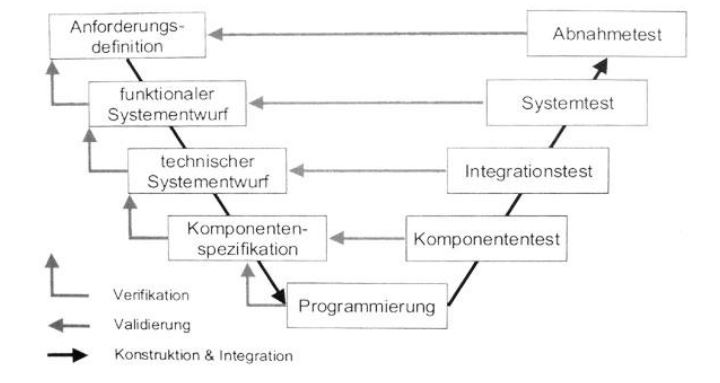
\includegraphics[scale=0.8]{img/vModell.jpg}\\
  \footnotesize\sffamily\textbf{Quelle:} \cite{spillner_basiswissen_2007}
  \caption{Allgemeines V-Modell}
  \label{fig:vModel}
\end{figure}


Die Aktivitäten des linke Astes lassen sich wie folgt beschreiben: \cite{spillner_basiswissen_2007}

\begin{itemize}
      \item \textbf{Anforderungsdefinition:} Die Wünsche und Anforderung des Auftraggebers oder späteren Systemanwenders werden gesammelt, spezifiziert und verabschiedet. Zweck und gewünschte Leistungsmerkmale des zu erstellenden Softwaresystems liegen damit fest.
      \item \textbf{Funktionaler Systementwurf:} Die Anforderungen werden auf Funktionen und Dialoge des neuen Systems abgebildet.
      \item \textbf{Technischer Systementwurf:} Die technische Realisierung des Systems wird entworfen. Hierzu gehören u.a.: Definition der Schnittstellen zur Systemumwelt und die Zerlegung des Systems in überschaubare Teilsysteme, die möglichst unabhängig voneinander entwickelt werden können.
      \item \textbf{Komponentenspezifikation:} Für jedes Teilsystem werden Aufgaben, Verhalten, innerer Aufbau und Schnittstellen zu anderen Teilsystemen definiert.
      \item \textbf{Programmierung:} Programmierung jedes spezifizierten Bausteins in einer Programmiersprache 
\end{itemize}


Der rechte Ast beschreibt zu den oben aufgeführten konstruktiven Aktivitäten eine korrespondierende Teststufe: \cite{spillner_basiswissen_2007}

\begin{itemize}
      \item \textbf{Komponententest:} Prüft, ob jeder einzelne Softwarebaustein für sich die Vorgaben seiner Spezifikation erfüllt.
      \item \textbf{Integrationstest:} Prüft, ob Gruppen von Komponenten wie im technischen Systementwurf vorgesehen zusammenspielen.
      \item \textbf{Systemtest:} Prüft, ob das System als Ganzes die spezifizierten Anforderungen erfüllt.
      \item \textbf{Abnahmetest:} Prüft, ob das System aus Kundensicht die vertraglich vereinbarten Leistungsmerkmale aufweist.
\end{itemize}
